\section{Results}
\label{sec:results}

\subsection{Productive AE4 loading requires an explicit alkalinity budget}
\label{sec:wt-reconstruction}

The conserved formulation separates productive chloride uptake from the acid--base cost of producing it. For the effective $1\Cl:1$ cation:$2\HCO$ cycle, inward chloride transport through AE4 removes two alkalinity equivalents. Carbon dioxide hydration redistributes carbonate species but does not create alkalinity. The balance therefore constrains the combined contributions of NHE1, AE2 and bicarbonate cotransport, not AE4 in isolation.

With the frozen NHE1 response and the stimulus recruited NBC-like pathway, the accepted wild type reconstruction sustains productive AE4 loading while maintaining the sampled physiological state. Its pH ranges from 6.9100 to 7.0348 over the 600 s stimulus. In the saved 60--600 s positive chloride loading budget, NKCC1 supplies 79.9248\% and AE4 supplies 20.0752\%; AE2 has no positive contribution in that interval. The signed time series in \cref{fig:chloride-loading} show that AE2 is slightly outward, rather than absent. The partition establishes a substantial AE4 contribution within this model; it is not an exact quantitative match to every pharmacological estimate of NKCC1's share.

The result supports the additional alkalinity pathway under the specified architecture and capacities. It does not establish a particular salivary NBC isoform, prove that all alternative sources of alkalinity are impossible, or imply that zero basal cotransport is a biological fact. Those stronger conclusions would require a broader model class and independent measurements.

\begin{figure}[t]
\centering
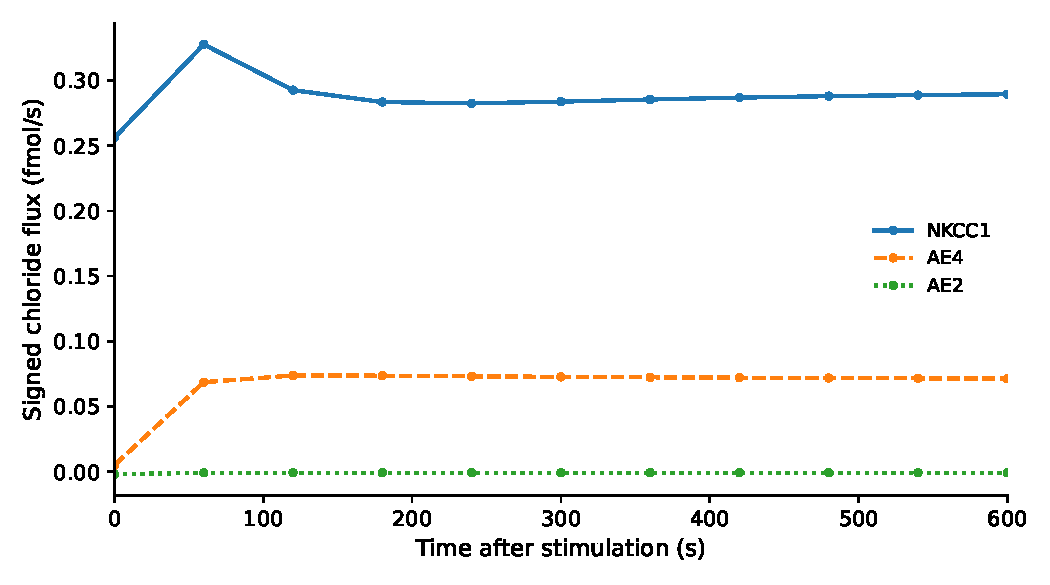
\includegraphics[width=\textwidth]{figures/fig01_chloride_loading.pdf}
\caption{Signed chloride loading in the accepted earlier wild type reconstruction. Points are the saved 60 s samples; joining segments do not resolve the early transient. NKCC1 and AE4 import chloride, while AE2 is slightly outward. The official 60--600 s positive loading fractions, 79.9248\% and 20.0752\%, are taken from the original integrated record, not recalculated from these coarse plotting samples.}
\label{fig:chloride-loading}
\end{figure}

\subsection{Later compensating networks conceal the effect of AE4 loss}
\label{sec:compensation}

Replacing the earlier NKCC representation by the Palk/Benjamin response produced strong compensation after acute AE4 removal. With donor weighted AE4 routing, the saved null trajectory increased integrated NKCC chloride loading by 33.10\% and reduced cumulative fluid secretion by only 0.627\%. Replacing the donor allocation by equal sodium and potassium routing reduced that compensation to 23.16\%, but the fluid deficit remained only 3.857\%. The corresponding 5\% AE4 expression case had a 3.418\% deficit. These are later reconstructions, not the behaviour of the original 2018 model, which reported weak NKCC activation.

The instantaneous NKCC ratios in \cref{fig:nkcc-compensation} show how the compensating response develops and persists. The percentage of normal chloride loading carried by AE4 is therefore not the percentage of secretion lost after AE4 deletion. Compensation changes the amount that reaches the apical membrane, and water secretion additionally depends on luminal composition and paracellular return.

For the equal routing source, this structural interaction is particularly transparent. Let $P=P_a+P_b$. Eliminating NKCC1, AE2 and NBC from the sodium, TA and chloride balances gives
\begin{equation}
 J_{Cl,a}=6P-J_H+2\dot n_{\mathrm{Na},i}-\dot n_{A,i}-\dot n_{\mathrm{Cl},i}.
 \label{eq:equal-routing-identity}
\end{equation}
At a stationary state, $J_{Cl,a}=6P-J_H$. The explicit AE4 term cancels, but the total response to AE4 loss does not: AE4 can still alter the state on which pump and NHE1 fluxes depend. This is neither a theorem of zero AE4 sensitivity nor a reason to apply the same reduced identity to the final donor weighted model. The general chloride reservoir identity in \cref{eq:reservoir-general} remains valid in both cases.

\begin{figure}[t]
\centering
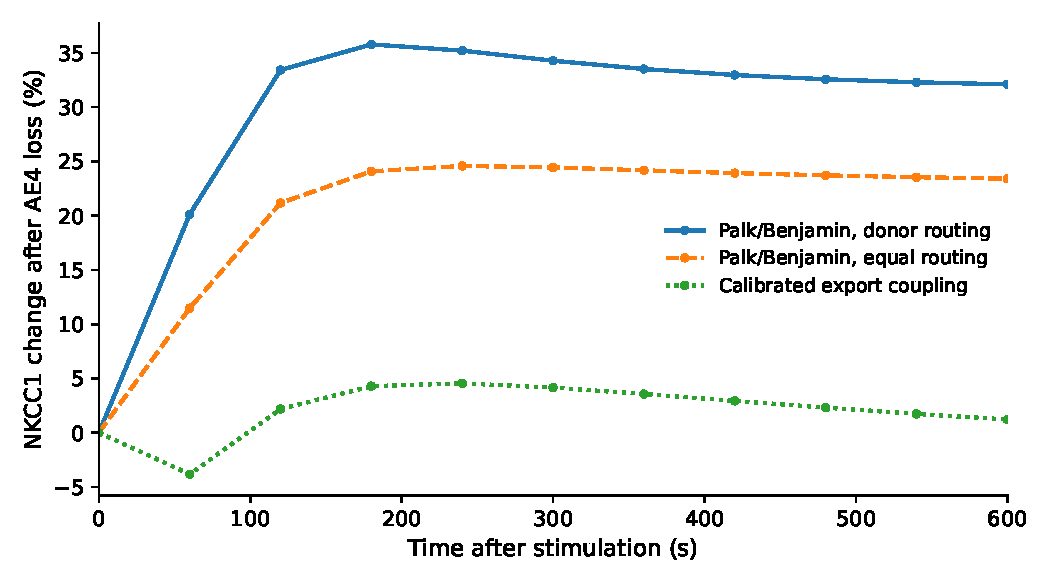
\includegraphics[width=\textwidth]{figures/fig02_nkcc_compensation.pdf}
\caption{Instantaneous NKCC1 chloride flux change after complete AE4 removal, $100(J_N^{\rm KO}/J_N^{\rm WT}-1)$, in three historical reconstructions. Each curve uses its own corresponding wild type and saved 60 s grid. These pointwise ratios are distinct from the reported integrated compensation values and do not simulate the experimental isolated NKCC assay. The export coupling is phenotype calibrated.}
\label{fig:nkcc-compensation}
\end{figure}

\subsection{Molecularly motivated source classes do not by themselves resolve the whole cell mechanism}
\label{sec:catalan-results}

The seven source classes in \cref{tab:mechanism-classes} passed source charge checks and admitted a resting wild type solution. Their predictions were fixed before the phenotype comparison. Eighteen of the 21 genotype trajectories passed the declared checks; the wild type carbonate classes C2, C4a and C4b instead crossed the lower pH limit at approximately 190, 222 and 317 s. Their saved traces end at the recorded failure in \cref{fig:class-ph}. A valid resting solution was not sufficient for physiological secretion.

Among classes with an admissible wild type reference, C1 predicted a 10.76\% \emph{increase} in knockout secretion and a 95.48\% increase in NKCC chloride loading. C3a predicted a 0.72\% secretion increase. The largest valid reduction was 7.67\% in C3b, whose proposed forward affinity was opposed at the reference state. These outcomes are summarised in \cref{tab:class-outcomes}; no failed wild type was replaced by an artificial 600 s endpoint.

\begin{table}[t]
\centering
\caption{Historical source-class outcomes with the inherited scalar kinetic law. Positive deficits mean less knockout fluid; negative values mean more. An absent endpoint is a physiological failure, not a prediction of zero secretion.}
\label{tab:class-outcomes}
\begin{tabularx}{\textwidth}{l r X}
\toprule
Class & Null deficit (\%) & Qualification\\
\midrule
C0 & 3.86 & Equal routing comparator; reference affinity opposed.\\
C1 & $-10.76$ & Valid trajectory; strong compensating NKCC response.\\
C2 & --- & Wild type pH failure at approximately 190 s.\\
C3a & $-0.72$ & Valid trajectory; little genotype separation.\\
C3b & 7.67 & Valid trajectory; reference affinity opposed.\\
C4a & --- & Wild type pH failure at approximately 222 s.\\
C4b & --- & Wild type pH failure at approximately 317 s.\\
\bottomrule
\end{tabularx}
\end{table}

This does not falsify the molecular transport mechanisms proposed by \citet{Catalan2025}. Each test changed the transported source coefficients while retaining an inherited scalar law. Where the new cycle affinity and that law disagree, the construction is not a fully thermodynamically matched kinetic model of the proposed mechanism. The defensible conclusion is that source-vector replacement alone did not produce a substantial, physiologically admissible deficit in this network. Carbonate removal also exposed the importance of distinguishing one carbon atom from two alkalinity equivalents.

\begin{figure}[t]
\centering
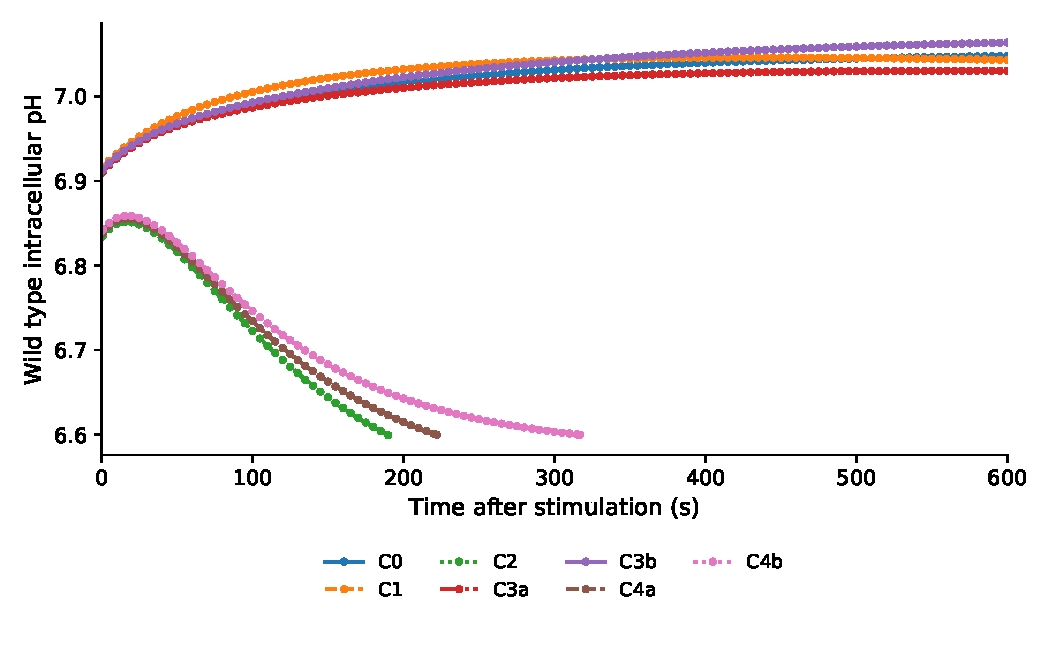
\includegraphics[width=\textwidth]{figures/fig03_class_ph.pdf}
\caption{Recorded wild type pH trajectories for the seven source classes. Curves use the stored samples and stop at their actual endpoints. C2, C4a and C4b reach the lower physiological gate near pH 6.6 before 600 s; the other four classes complete the protocol. Charge neutrality and a resting solution do not prevent a later acid--base failure.}
\label{fig:class-ph}
\end{figure}

\subsection{An effective apical coupling establishes sufficiency, not molecular necessity}
\label{sec:calibrated-coupling}

A separate inverse construction reduced stimulated apical chloride conductance as AE4 expression decreased. Its compact beta conditioned form is
\begin{equation}
 G_{Cl}^{\rm eff}=G_{Cl}^{\rm parent}
 \bigl[1-\lambda a_{Ca}\beta(1-e_4)\bigr],
 \qquad \lambda=0.89488127156712.
 \label{eq:calibrated-coupling}
\end{equation}
Here $a_{Ca}$ is the existing normalised calcium activation and $e_4$ is AE4 expression. Wild type, zero beta input and the resting increment retain their parent vector fields. The coefficient is inherited from phenotype calibration, not measured channel biology. The combined-protocol results are reused from the frozen accepted benchmark with the documented numerical equivalence qualification for coefficient rounding; they are not new integrations.

At full activation, knockout conductance is approximately 10.51\% of its parent value. This strong interaction yields a 30.261\% cumulative null deficit and a 23.163\% deficit at 5\% AE4 expression, while passing the declared 600 s checks. Integrated NKCC compensation falls to approximately 2.79\% in the null. The construction proves that a network interaction can generate a large deficit without eliminating other transporters. It does not prove direct AE4 regulation of TMEM16A, distinguish channel trafficking from another effective interaction, or establish that such a multiplier is required by all alternative explanations.

The temporal comparison in \cref{fig:cumulative-deficits} separates this calibrated benchmark from the small deficit of the compensating model and the final reservoir result. No experimental 600 s percentage is drawn as a band over every earlier time. The trajectory shapes are predictions of their respective assumptions, not fits to minute specific observations.

\begin{figure}[t]
\centering
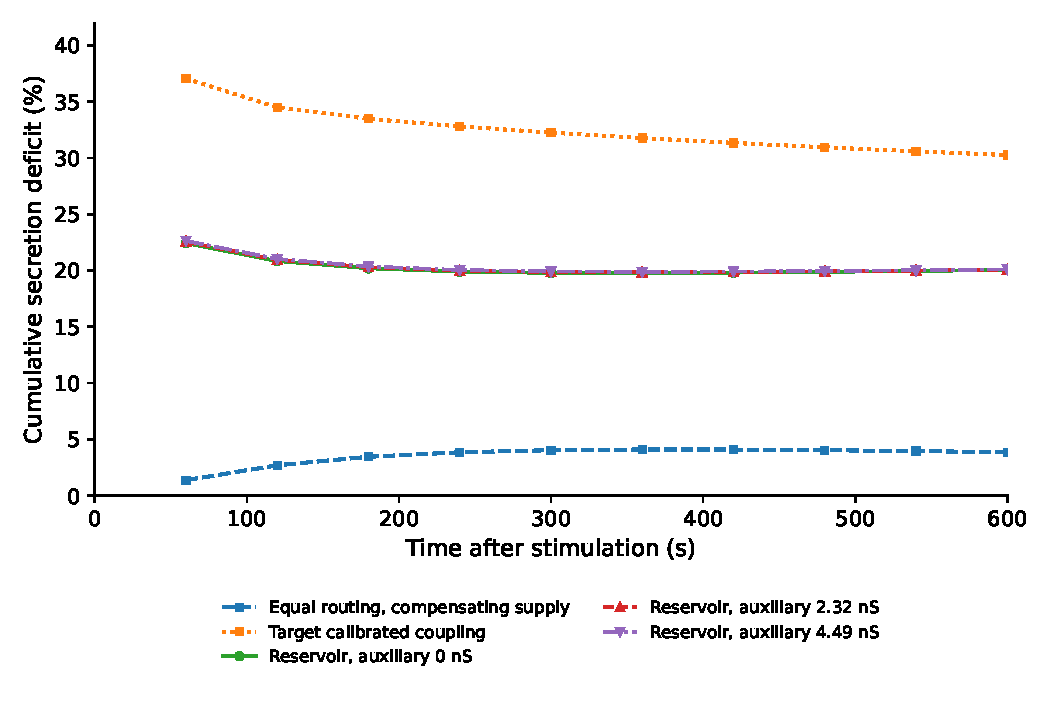
\includegraphics[width=\textwidth]{figures/fig04_cumulative_deficits.pdf}
\caption{Cumulative fluid deficit, $100[1-Q_{\rm KO}(t)/Q_{\rm WT}(t)]$, at the ten declared observation times. The compensating equal routing model gives a small effect; the target calibrated apical coupling gives a larger one. The three final reservoir curves nearly coincide despite different shared auxiliary conductances. Each construction uses its own corresponding wild type. Joining lines connect recorded integral summaries, not newly fitted trajectories.}
\label{fig:cumulative-deficits}
\end{figure}

\subsection{Shared secretory demand reveals the chloride availability difference}
\label{sec:reservoir-result}

The final paired comparison produces a substantial secretion difference without \cref{eq:calibrated-coupling}. All three central cases reach 600 s and pass their frozen sampled physical and conservation checks. Cumulative fluid deficits are 20.039\%, 20.076\% and 20.102\% for auxiliary conductances 0, 2.32 and 4.49 nS, respectively. The range across these alternatives is only 0.062 percentage points. Thus this particular conductance choice is not creating the genotype separation.

At 2.32 nS, wild type secretes 0.978612 pL and knockout 0.782148 pL over 600 s. The mean-flow deficit over 60--600 s is 19.788\%, and the endpoint flow deficit is 20.899\%. The cumulative difference is therefore not a brief effect selected at a favourable observation time. The absolute flow traces are shown in \cref{fig:fluid-flow}; their early transient is not independently calibrated to experimental timing.

\begin{table}[t]
\centering
\caption{Verified central paired outcomes over 0--600 s. Fluid and apical chloride totals use the original headline trapezoidal rule. These are model cell outputs, not absolute whole gland volumes.}
\label{tab:central-results}
\begin{tabular}{rrrrr}
\toprule
$G_{\rm aux}$ & WT fluid & KO fluid & Fluid deficit & Cl export deficit\\
(nS) & (pL) & (pL) & (\%) & (\%)\\
\midrule
0 & 0.972955 & 0.777980 & 20.039 & 18.208\\
2.32 & 0.978612 & 0.782148 & 20.076 & 18.232\\
4.49 & 0.982744 & 0.785197 & 20.102 & 18.249\\
\bottomrule
\end{tabular}
\end{table}

\begin{figure}[t]
\centering
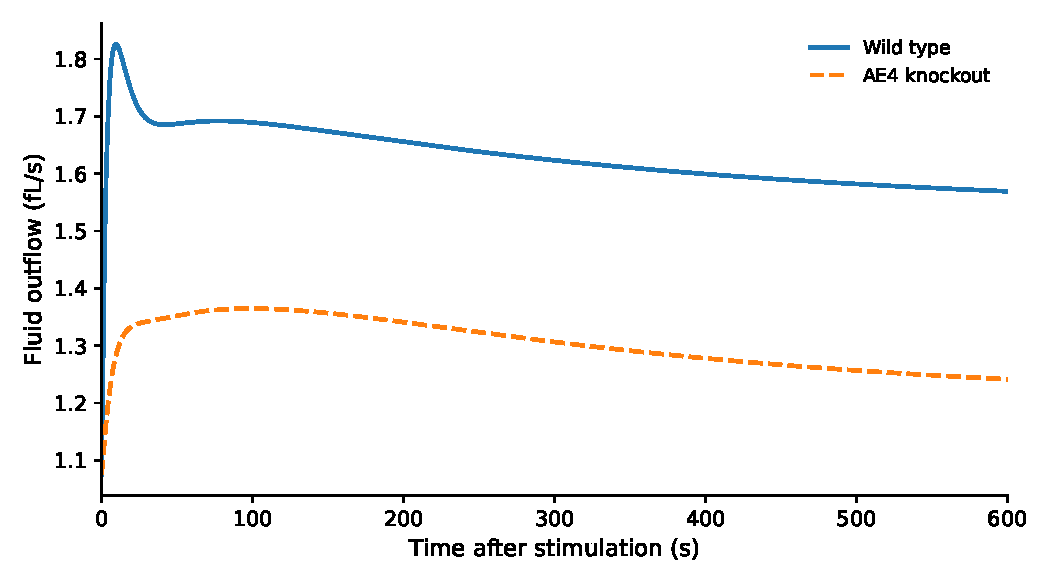
\includegraphics[width=\textwidth]{figures/fig05_fluid_flow.pdf}
\caption{Fluid outflow for the central 2.32 nS shared auxiliary conductance. The knockout has lower flow over the sustained response despite identical prescribed NKCC1 and AE2 supply and identical channel parameters. The curves use saved accepted-step and integer-second samples, including the separate onset convention.}
\label{fig:fluid-flow}
\end{figure}

Wild type retains a larger intracellular chloride concentration throughout the recorded response (\cref{fig:chloride}). Both concentrations initially rise before declining; the mechanism is not complete exhaustion of a fixed chloride store. Wild type continues to load chloride through AE4 while the knockout cannot. At 600 s the central concentrations are approximately 53.71 and 37.50 mM. The associated pH values are 7.029 and 7.274. These later states are predictions conditional on the projection and supply construction, not imposed measurements.

\begin{figure}[t]
\centering
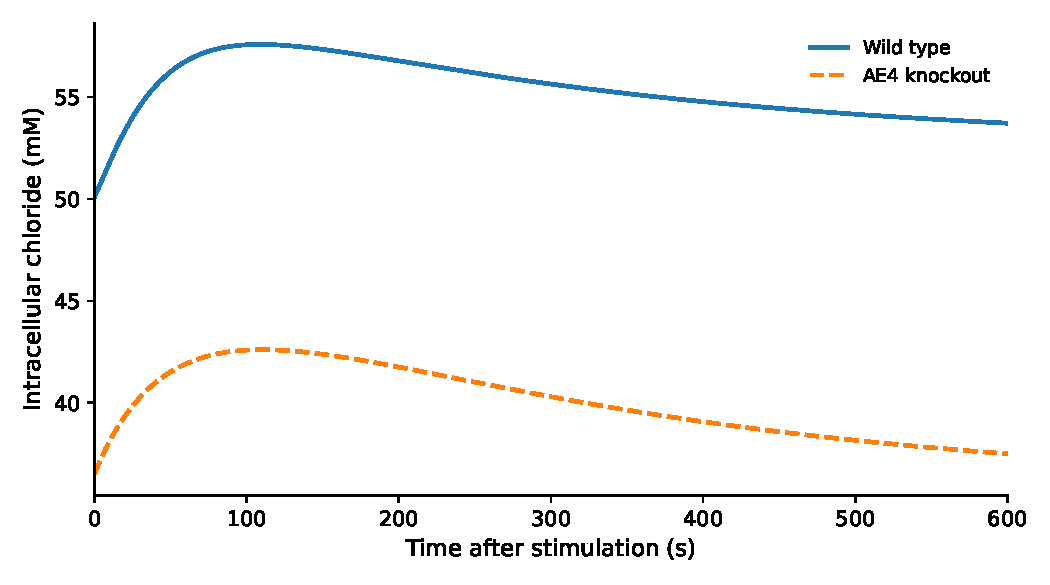
\includegraphics[width=\textwidth]{figures/fig06_chloride.pdf}
\caption{Intracellular chloride in the same central pair. Only the onset chloride values are imposed from the genotype measurements. The subsequent rise and decline are recorded model dynamics. The persistent difference accompanies continuing wild type AE4 supply; it should not be interpreted as simple emptying of the initial store.}
\label{fig:chloride}
\end{figure}

\subsection{The conserved budget accounts for the additional wild type export}
\label{sec:budget-result}

For the central 2.32 nS case, the initial wild type chloride advantage is 19.698595 fmol. Continuing AE4 input contributes another 46.652418 fmol, and 24.487456 fmol of intracellular difference remains at 600 s. Equation~\eqref{eq:reservoir-matched} therefore accounts for 41.863556 fmol of extra wild type apical export. Differential NKCC1 and AE2 contributions are exactly zero by construction. The numerical reconstruction and the independently integrated export are indistinguishable at the figure scale in \cref{fig:reservoir-budget}.

\begin{table}[t]
\centering
\caption{Independent chloride budget using saved Gauss quadrature, including the separately recorded onset term. All amounts are fmol. The two matched non-AE4 supply differences are zero. The last column is the absolute endpoint error in \cref{eq:reservoir-matched}, not an error inferred from the coarse plotting grid.}
\label{tab:budget}
\begin{tabular}{rrrrrr}
\toprule
$G_{\rm aux}$ (nS) & $\delta(0)$ & $D_4$ & $\delta(600)$ & $D_{Cl,a}$ & Error\\
\midrule
0 & 19.698595 & 46.636713 & 24.735190 & 41.600118 & $6.87\times10^{-8}$\\
2.32 & 19.698595 & 46.652418 & 24.487456 & 41.863556 & $7.23\times10^{-8}$\\
4.49 & 19.698595 & 46.663679 & 24.307622 & 42.054652 & $7.49\times10^{-8}$\\
\bottomrule
\end{tabular}
\end{table}

\begin{figure}[t]
\centering
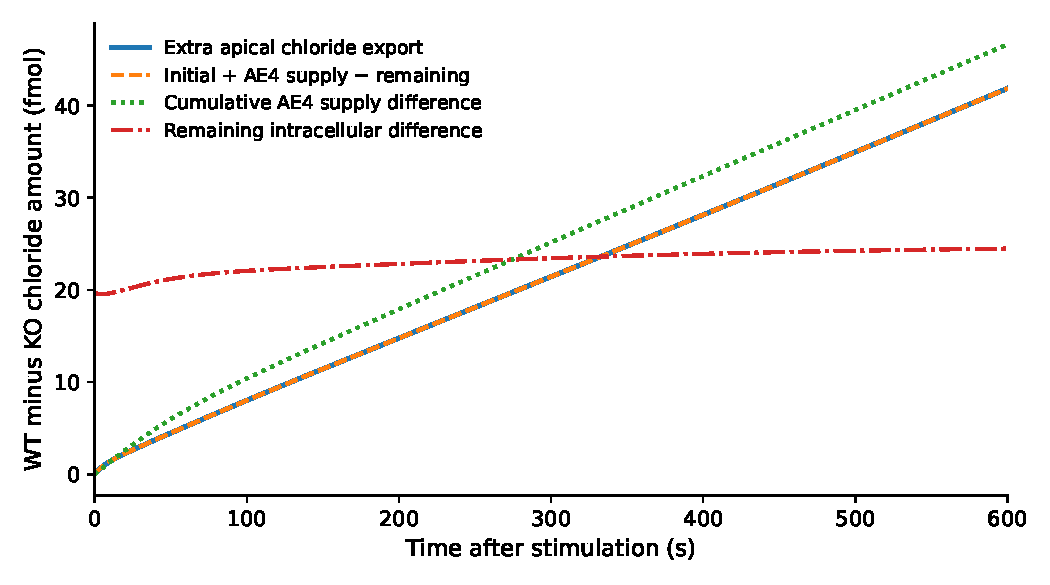
\includegraphics[width=\textwidth]{figures/fig07_reservoir_budget.pdf}
\caption{Time resolved chloride accounting for the central pair. The independently saved extra apical export overlays its mass balance reconstruction, $\delta(0)+D_4(t)-\delta(t)$. The other curves show cumulative AE4 supply and the remaining intracellular difference. Values use the original accepted-step Gauss integrals plus the documented onset contribution; no flux integral is inferred from the state difference.}
\label{fig:reservoir-budget}
\end{figure}

The endpoint errors across all three cases are below $7.5\times10^{-8}$ fmol, compared with the predeclared $10^{-5}$ fmol tolerance. The central headline chloride export deficit is approximately 18.23\%, while its fluid deficit is 20.08\%. Their difference is expected: apical export, net chloride outflow and water outflow are different observables. Exact chloride accounting establishes how much substrate is available to the secretory route, not a universal fixed conversion from exported chloride to fluid volume.

The shared conductance has a smaller driving force in knockout (\cref{fig:driving-force}). At 600 s, the central outward chloride driving forces are approximately 2.03 mV in wild type and 1.60 mV in knockout. Thus equal channel parameters need not give equal chloride currents. This supplies the physical connection between a shared demand pathway and genotype dependent output without an AE4 specific conductance coefficient.

\begin{figure}[t]
\centering
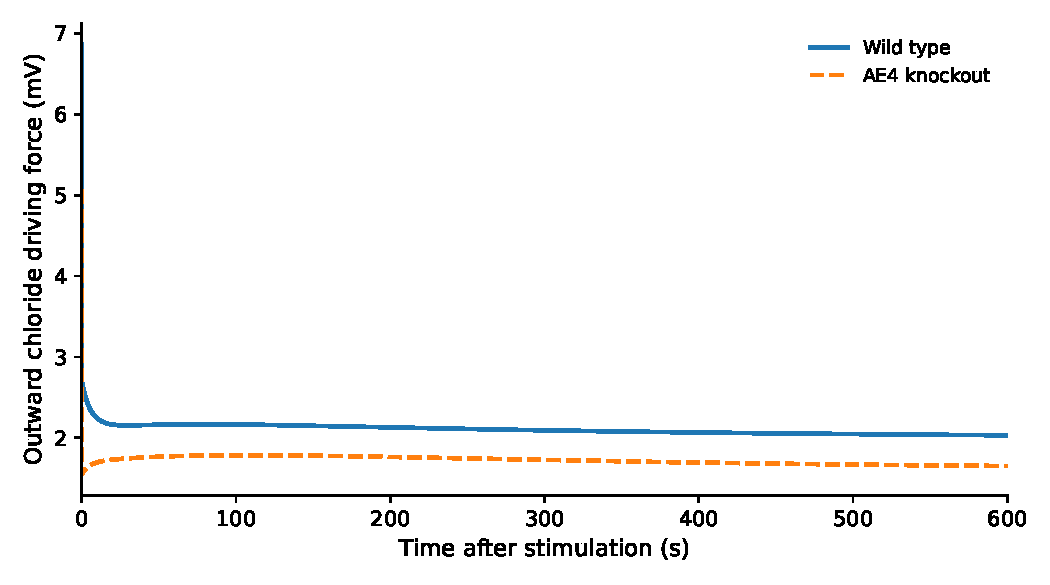
\includegraphics[width=\textwidth]{figures/fig08_driving_force.pdf}
\caption{Outward chloride driving force, $E_{\rm Cl}-V_a$, for the central pair. Identical conductance parameters act on different evolving electrochemical states. The early jump follows the prescribed stimulus convention and is not a fitted experimental onset.}
\label{fig:driving-force}
\end{figure}

\subsection{Reported sensitivities delimit the interpretation}
\label{sec:reported-sensitivities}

The manuscript continuation record reports the outcomes in \cref{tab:reported-sensitivities}. Increasing knockout non-AE4 supply by 5\% or 10\% attenuated, rather than reversed, the deficit. An alternate onset projection gave a similar central magnitude. However, the CCh only result retained much of the effect, and the IPR only trajectory failed the frozen knockout pH check before 600 s. These outcomes are useful qualifications, but their underlying arrays were not available for the independent file checks performed in this manuscript revision. They are deliberately not drawn as time series.

\begin{table}[t]
\centering
\caption{Reported continuation summaries, not independently reverified trajectories in this revision. Values are approximate as preserved in the manuscript decision record. The IPR failure has no valid 600 s secretion endpoint.}
\label{tab:reported-sensitivities}
\begin{tabularx}{\textwidth}{l r X}
\toprule
Comparison & Fluid deficit (\%) & Interpretation of reported outcome\\
\midrule
KO non-AE4 supply $\times1.05$ & 17.65 & Added supply attenuates the effect.\\
KO non-AE4 supply $\times1.10$ & 15.30 & Direction retained under the larger perturbation.\\
Alternate onset projection & 19.77 & Similar magnitude with a different projected state.\\
CCh only & 18.92 & Beta specificity is not established.\\
IPR only & --- & KO pH gate reached at approximately 488 s.\\
\bottomrule
\end{tabularx}
\end{table}

\subsection{Comparison with the original explanation}

The original model, the later compensating network, the calibrated interaction and the reservoir comparison answer different questions (\cref{tab:model-comparison}). The final comparison does not recover the original sodium/pump explanation unchanged. It demonstrates instead that a substantial chloride availability difference can be expressed through otherwise shared secretory pathways. That conclusion is conditional on the projected state and prescribed supply. The conserved accounting is exact; the biological identification of those assumptions is not.

\begin{table}[t]
\centering
\caption{What the main model comparisons establish. Scalar outcomes are kept in a table because no original-model time series is manufactured for this revision. Percentages are not interchangeable fractions of the same mechanism.}
\label{tab:model-comparison}
\begin{tabularx}{\textwidth}{p{0.23\textwidth}rX}
\toprule
Construction & Null deficit & Scientific status\\
\midrule
Original 2018 model & $\sim24\%$ & Cation coupled explanation in the original acid--base and transport network.\\
Later Palk/Benjamin, donor routing & $0.63\%$ & Strong state dependent NKCC compensation.\\
Later equal routing & $3.86\%$ & Small effect despite appreciable WT AE4 loading.\\
Calibrated apical interaction & $30.26\%$ & Proof of sufficiency with a phenotype selected coefficient.\\
Final chloride availability comparison & $20.04$--$20.10\%$ & Conditional mechanism with measured onset constraints and prescribed matched supply.\\
\bottomrule
\end{tabularx}
\end{table}
